%% ============================================================
%% MRI Digital Twin — Siemens Healthineers
%% Landscape Beamer Presentation  |  June 2026
%% ============================================================
\documentclass[aspectratio=169,12pt]{beamer}

%% ---- Theme ----
\usetheme{metropolis}

%% ---- Packages ----
\usepackage{fontspec}
\setsansfont{Liberation Sans}[Scale=MatchLowercase]
\setmonofont{Liberation Mono}[Scale=MatchLowercase]
\usepackage{graphicx}
\usepackage{booktabs}
\usepackage{xcolor}
\usepackage{tikz}
\usetikzlibrary{calc}
\usepackage{array}
\usepackage{colortbl}
\usepackage{microtype}
\usepackage{amsmath}
\usepackage{hyperref}

\graphicspath{{figures/}}

%% ---- Siemens Healthineers Colour Palette ----
\definecolor{SiemensTeal}{RGB}{0,153,153}
\definecolor{SiemensNavy}{RGB}{0,48,135}
\definecolor{SiemensOrange}{RGB}{236,102,2}
\definecolor{SiemensLight}{RGB}{240,247,247}
\definecolor{SiemensMid}{RGB}{204,238,238}
\definecolor{SiemensDark}{RGB}{26,26,26}
\definecolor{SiemensMuted}{RGB}{107,123,123}

%% ---- Theme Overrides ----
\setbeamercolor{normal text}{fg=SiemensDark,bg=white}
\setbeamercolor{alerted text}{fg=SiemensOrange}
\setbeamercolor{example text}{fg=SiemensTeal}
\setbeamercolor{frametitle}{bg=SiemensNavy,fg=white}
\setbeamercolor{title separator}{fg=SiemensTeal}
\setbeamercolor{progress bar}{fg=SiemensTeal,bg=SiemensMid}
\setbeamercolor{section in toc}{fg=SiemensNavy}
\setbeamercolor{section page}{bg=SiemensNavy,fg=white}
\setbeamercolor{palette primary}{fg=white,bg=SiemensNavy}
\setbeamercolor{block title}{bg=SiemensNavy,fg=white}
\setbeamercolor{block body}{bg=SiemensLight,fg=SiemensDark}
\setbeamercolor{block title alerted}{bg=SiemensOrange,fg=white}
\setbeamercolor{block body alerted}{bg=SiemensLight,fg=SiemensDark}
\setbeamercolor{block title example}{bg=SiemensTeal,fg=white}
\setbeamercolor{block body example}{bg=SiemensLight,fg=SiemensDark}

\metroset{titleformat=regular,progressbar=frametitle,block=fill,sectionpage=none}

%% ---- Custom section separator slides ----
\AtBeginSection{%
  \begin{frame}[plain]
    \begin{tikzpicture}[remember picture, overlay]
      %% Full navy background
      \fill[SiemensNavy] (current page.south west) rectangle (current page.north east);
      %% Teal accent bar — left edge, full height
      \fill[SiemensTeal] (current page.south west) rectangle ($(current page.north west)+(0.28,0)$);
      %% Subtle light band across middle
      \fill[white,opacity=0.04]
        ($(current page.west)+(0,-0.9)$) rectangle ($(current page.east)+(0,0.9)$);
      %% Decorative circle — upper right
      \draw[SiemensTeal,line width=1.2pt,opacity=0.35]
        ($(current page.north east)+(-1.4,-1.4)$) circle (2.2cm);
      \draw[SiemensTeal,line width=0.6pt,opacity=0.2]
        ($(current page.north east)+(-1.4,-1.4)$) circle (3.2cm);
      %% Section number pill
      \node[fill=SiemensTeal,rounded corners=4pt,
            text=white,font=\bfseries\large,
            inner xsep=10pt,inner ysep=5pt]
        at ($(current page.west)+(2.8,0.55)$)
        {\insertsectionnumber};
      %% Section title
      \node[text=white,font=\bfseries\LARGE,
            text width=12cm,align=left]
        at ($(current page.center)+(1.2,0)$)
        {\insertsectionhead};
      %% Thin teal line under title
      \draw[SiemensTeal,line width=1.5pt]
        ($(current page.center)+(-3.8,-0.75)$) --
        ($(current page.center)+(6.2,-0.75)$);
    \end{tikzpicture}
  \end{frame}%
}

%% ---- Helper: coloured rule ----
\newcommand{\tealsep}{\vspace{1pt}\textcolor{SiemensTeal}{\rule{\linewidth}{1pt}}\vspace{4pt}}
\newcommand{\navysep}{\vspace{1pt}\textcolor{SiemensNavy}{\rule{\linewidth}{0.6pt}}\vspace{3pt}}

%% ---- Title info ----
\title{MRI Digital Twin}
\subtitle{Generative Simulation \& Semantic Intelligence for Siemens Healthineers}
\author{Customer Twin Project Team \quad\textcolor{SiemensTeal}{$\cdot$}\quad Siemens Healthineers}
\date{June 2026}
\institute{}

%% ============================================================
\begin{document}

%% ----------------------------------------------------------
%% SLIDE 1 — Title
%% ----------------------------------------------------------
\begin{frame}[plain,noframenumbering]
  \begin{tikzpicture}[remember picture, overlay]
    \fill[SiemensNavy] (current page.south west) rectangle (current page.north east);
    \fill[SiemensTeal] (current page.south west) rectangle ($(current page.north west)+(0.35,0)$);
    \draw[SiemensTeal,line width=1pt,opacity=0.3]
      ($(current page.north east)+(-1.8,-1.8)$) circle (2.6cm);
    \draw[SiemensTeal,line width=0.5pt,opacity=0.18]
      ($(current page.north east)+(-1.8,-1.8)$) circle (3.8cm);
  \end{tikzpicture}
  \vspace{1.6cm}
  \centering
  {\color{white}\fontsize{26}{30}\selectfont\bfseries MRI Digital Twin}\par\vspace{0.4cm}
  {\color{SiemensTeal}\fontsize{12}{15}\selectfont Generative Simulation \& Semantic Intelligence for Siemens Healthineers}\par\vspace{0.7cm}
  \textcolor{white!70!SiemensNavy}{\small Customer Twin Project Team \quad\textcolor{SiemensTeal}{$\cdot$}\quad Siemens Healthineers}\par\vspace{0.2cm}
  \textcolor{SiemensMuted}{\small June 2026}
\end{frame}

%% ----------------------------------------------------------
%% SLIDE 2 — Agenda
%% ----------------------------------------------------------
\begin{frame}[shrink=5]{Agenda}
\vspace{-6pt}
\tealsep
\begin{columns}[T]
\column{0.48\textwidth}
\begin{enumerate}\setlength\itemsep{2pt}
  \item[\textcolor{SiemensTeal}{\textbf{1.}}] \textbf{Strategic Context} — The Four Twins mandate
  \item[\textcolor{SiemensTeal}{\textbf{2.}}] \textbf{The Problem} — Cost of scheduling inefficiency
  \item[\textcolor{SiemensTeal}{\textbf{3.}}] \textbf{What We're Building} — The Customer Twin
  \item[\textcolor{SiemensTeal}{\textbf{4.}}] \textbf{Technical Architecture} — Models \& pipeline
  \item[\textcolor{SiemensTeal}{\textbf{5.}}] \textbf{MRRT Insight Agent} — Semantic intelligence
\end{enumerate}
\column{0.48\textwidth}
\begin{enumerate}\setlength\itemsep{2pt}
  \item[\textcolor{SiemensOrange}{\textbf{6.}}] \textbf{Current Status} — What's built \& running
  \item[\textcolor{SiemensOrange}{\textbf{7.}}] \textbf{Demonstrated Results} — Validation evidence
  \item[\textcolor{SiemensOrange}{\textbf{8.}}] \textbf{How Things Are Run} — Infrastructure
  \item[\textcolor{SiemensOrange}{\textbf{9.}}] \textbf{Roadmap} — Next steps \& milestones
  \item[\textcolor{SiemensOrange}{\textbf{10.}}] \textbf{Financial Impact} — ROI per machine
\end{enumerate}
\end{columns}
\end{frame}

%% ===========================================================
\section{Strategic Context}
%% ===========================================================

%% ----------------------------------------------------------
%% SLIDE 3 — The Four Twins
%% ----------------------------------------------------------
\begin{frame}{The Four Twins Ecosystem}
\vspace{-6pt}
\begin{center}
  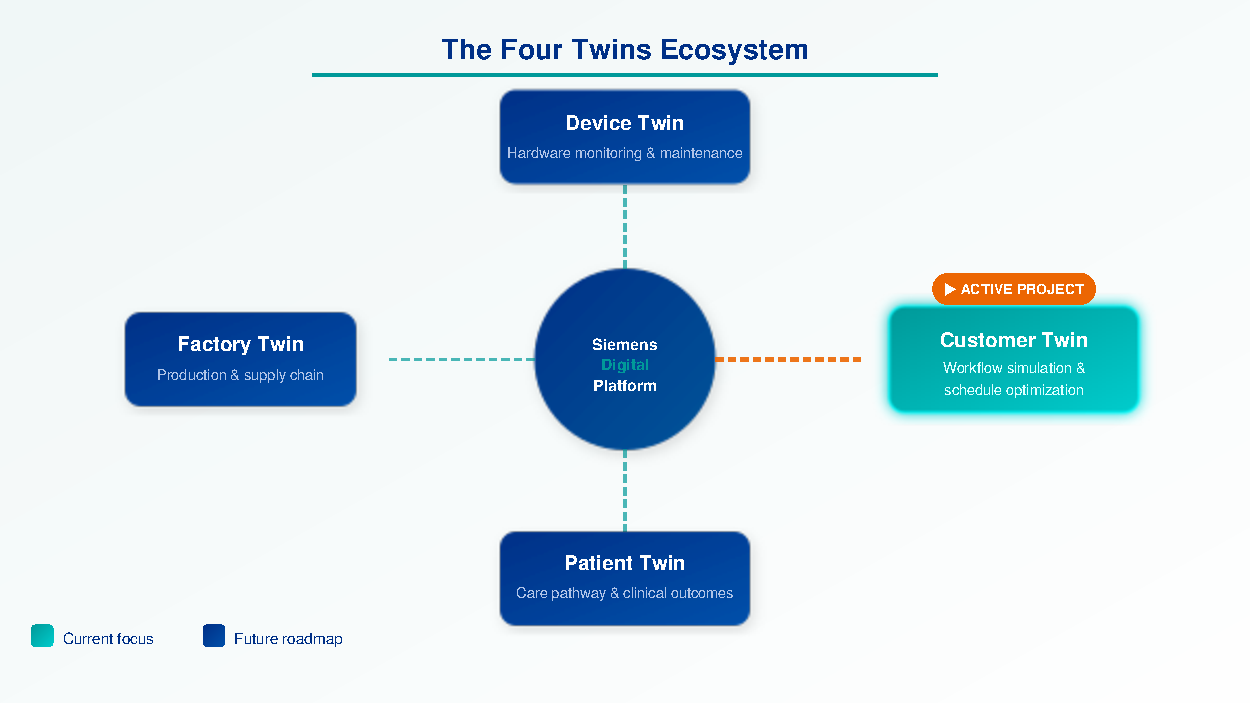
\includegraphics[width=\textwidth,height=0.82\textheight,keepaspectratio]{01-four-twins}
\end{center}
\end{frame}

%% ----------------------------------------------------------
%% SLIDE 4 — From Reporting to Simulation
%% ----------------------------------------------------------
\begin{frame}[shrink=15]{From Reporting to Simulation}
\tealsep
\begin{columns}[T]
\column{0.46\textwidth}
\begin{block}{Today — Static Reporting}
\begin{itemize}\setlength\itemsep{4pt}
  \item Manual scheduling based on fixed slot durations
  \item Post-hoc reports on downtime and utilisation
  \item Reactive maintenance after hardware failure
  \item No forward-looking capacity simulation
  \item Coil/hardware ROI assessed only after purchase
\end{itemize}
\end{block}

\column{0.46\textwidth}
\begin{exampleblock}{Tomorrow — Generative Simulation}
\begin{itemize}\setlength\itemsep{4pt}
  \item \textbf{Generative AI} produces synthetic daily schedules
  \item Real-time uncertainty bounds $\boldsymbol{\mu \pm \sigma}$ per scan
  \item Predictive maintenance — \textbf{2 weeks} advance warning
  \item Pre-purchase ROI modelling for hardware upgrades
  \item VR training without occupying a live scanner
\end{itemize}
\end{exampleblock}
\end{columns}
\vspace{6pt}
\textcolor{SiemensMuted}{\footnotesize This transition is the strategic mandate of the Siemens Healthineers \emph{Four Twins} programme.}
\end{frame}

%% ===========================================================
\section{The Problem}
%% ===========================================================

%% ----------------------------------------------------------
%% SLIDE 5 — The Scheduling Challenge
%% ----------------------------------------------------------
\begin{frame}[shrink=20]{The Scheduling Challenge}
\tealsep
\begin{columns}[T]
\column{0.55\textwidth}
\textbf{MRI scan durations are inherently unpredictable:}
\vspace{6pt}
\begin{itemize}\setlength\itemsep{6pt}
  \item A single scanner serves scans ranging from \alert{\textbf{30 seconds to 45 minutes}}
  \item Static appointment slots cannot adapt to this variance
  \item One overrun cascades — delays ripple through the entire day
  \item Clinical priority (urgent vs routine) further disrupts static queues
  \item Technician workload spikes unpredictably at coil changes
\end{itemize}
\vspace{8pt}
\begin{alertblock}{The Root Cause}
  Static scheduling treats stochastic processes as deterministic — the wrong model for MRI workflows.
\end{alertblock}

\column{0.40\textwidth}
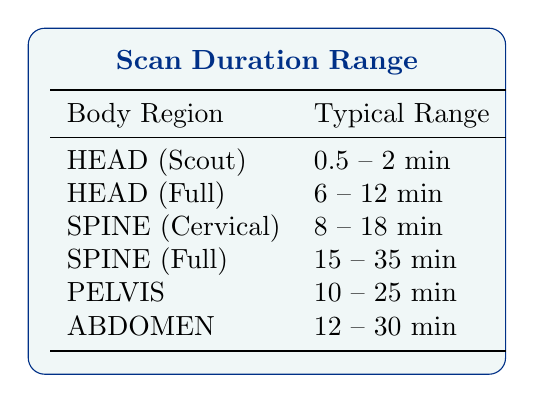
\begin{tikzpicture}
  \node[draw=SiemensNavy,fill=SiemensLight,rounded corners=6pt,
        text width=5.5cm,align=center,inner sep=8pt] at (0,0) {%
    \textcolor{SiemensNavy}{\textbf{Scan Duration Range}}\\[4pt]
    \begin{tabular}{ll}
      \toprule
      Body Region & Typical Range \\
      \midrule
      HEAD (Scout)    & $0.5$ -- $2$ min \\
      HEAD (Full)     & $6$ -- $12$ min  \\
      SPINE (Cervical) & $8$ -- $18$ min \\
      SPINE (Full)    & $15$ -- $35$ min \\
      PELVIS          & $10$ -- $25$ min \\
      ABDOMEN         & $12$ -- $30$ min \\
      \bottomrule
    \end{tabular}%
  };
\end{tikzpicture}
\end{columns}
\end{frame}

%% ----------------------------------------------------------
%% SLIDE 6 — The Hidden Cost
%% ----------------------------------------------------------
\begin{frame}{The Hidden Cost of Inefficiency}
\vspace{-6pt}
\begin{center}
  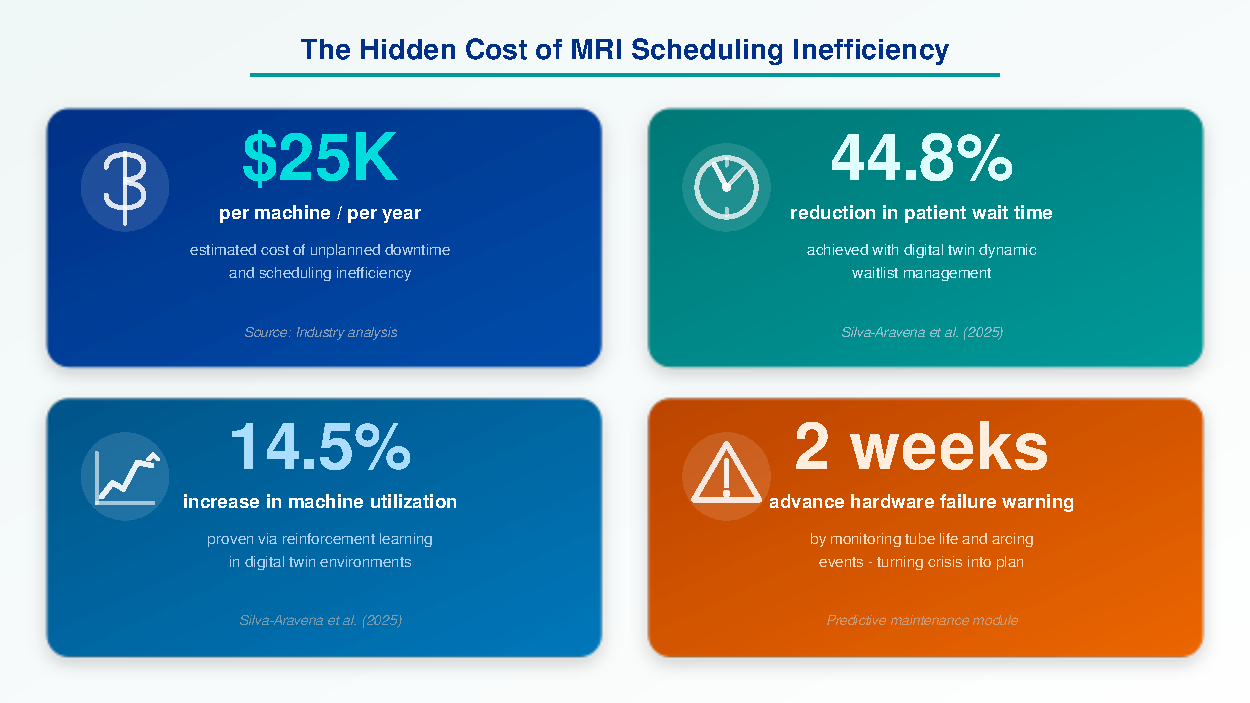
\includegraphics[width=\textwidth,height=0.84\textheight,keepaspectratio]{02-problem-stats}
\end{center}
\end{frame}

%% ----------------------------------------------------------
%% SLIDE 7 — What's Missing
%% ----------------------------------------------------------
\begin{frame}[shrink=12]{What's Missing — and What We Provide}
\tealsep
\vspace{4pt}
\begin{tabular}{p{0.28\linewidth}p{0.30\linewidth}p{0.30\linewidth}}
\rowcolor{SiemensNavy}
\textcolor{white}{\textbf{Current State}} &
\textcolor{white}{\textbf{What's Needed}} &
\textcolor{SiemensTeal}{\textbf{What We Build}} \\[2pt]
\rowcolor{SiemensLight}
Manual, fixed-slot scheduling & Dynamic scheduling based on real-time simulation &
\textcolor{SiemensTeal}{Generative synthetic day with $\mu \pm \sigma$ per slot} \\[4pt]
\rowcolor{white}
Reactive maintenance after failure & 2-week advance hardware failure warning &
\textcolor{SiemensTeal}{Tube life + arcing signal monitoring model} \\[4pt]
\rowcolor{SiemensLight}
Post-hoc utilisation reports & Forward-looking capacity simulation &
\textcolor{SiemensTeal}{Customer Twin: simulate any future day} \\[4pt]
\rowcolor{white}
Coil ROI guessed at point-of-sale & Pre-purchase ROI simulation per site &
\textcolor{SiemensTeal}{Counterfactual day simulation with/without upgrade} \\[4pt]
\rowcolor{SiemensLight}
Paper-based technician training & Immersive VR practice environment &
\textcolor{SiemensTeal}{Unity / Meta Quest simulation from digital twin} \\[4pt]
\rowcolor{white}
Manual R\&D feedback triage & Automated semantic pain extraction &
\textcolor{SiemensTeal}{MRRT LLM Insight Agent over customer comments} \\
\end{tabular}
\end{frame}

%% ===========================================================
\section{What We're Building}
%% ===========================================================

%% ----------------------------------------------------------
%% SLIDE 8 — The Customer Twin
%% ----------------------------------------------------------
\begin{frame}{The Customer Twin — System Overview}
\vspace{-6pt}
\begin{center}
  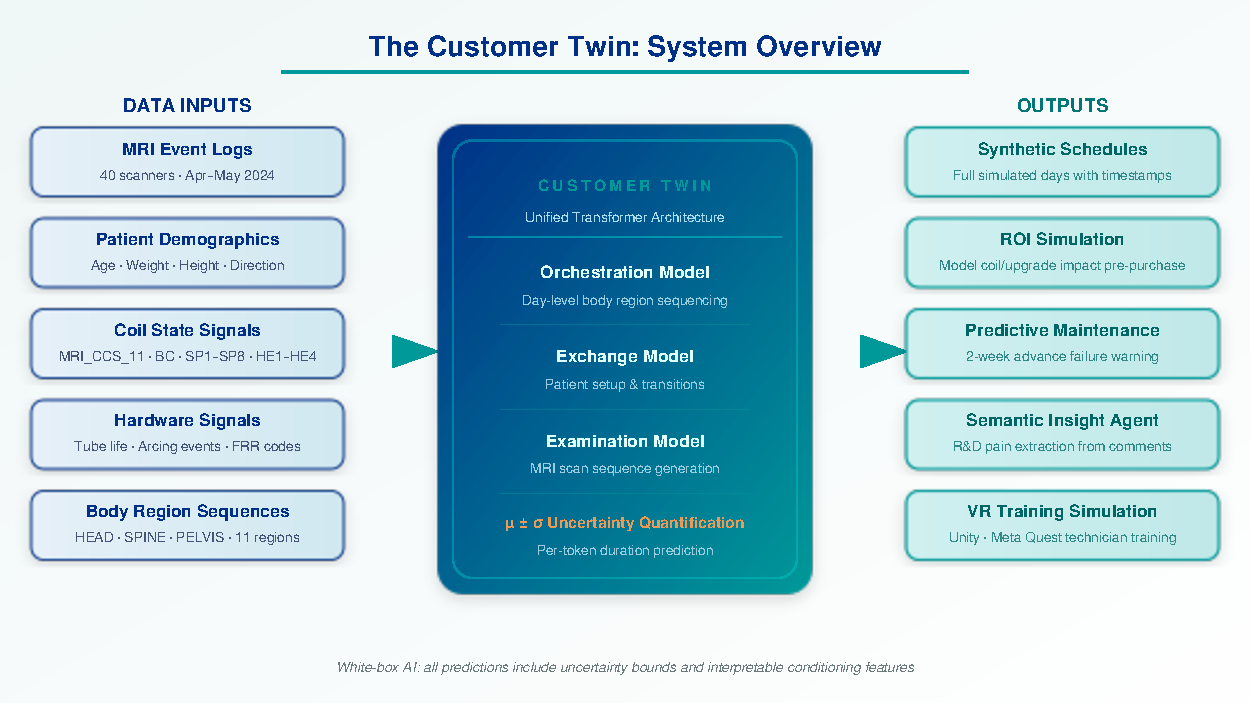
\includegraphics[width=\textwidth,height=0.84\textheight,keepaspectratio]{03-customer-twin-overview}
\end{center}
\end{frame}

%% ----------------------------------------------------------
%% SLIDE 9 — Three Parallel Workstreams
%% ----------------------------------------------------------
\begin{frame}[shrink=20]{Three Parallel Workstreams}
\tealsep
\begin{columns}[T]
\column{0.30\textwidth}
\begin{block}{\textbf{1.} Alternating Pipeline}
  \begin{itemize}\setlength\itemsep{4pt}
    \item Generative transformer models
    \item Exchange + Examination alternation
    \item Orchestrator for day sequencing
    \item $\mu \pm \sigma$ duration per token
    \item Output: full synthetic day CSV
  \end{itemize}
\end{block}

\column{0.30\textwidth}
\begin{exampleblock}{\textbf{2.} MRRT Insight Agent}
  \begin{itemize}\setlength\itemsep{4pt}
    \item LLM-based semantic search
    \item Corpus: unstructured customer comments
    \item Identifies coil positioning friction
    \item Extracts R\&D ``pains'' at scale
    \item Structured output for product teams
  \end{itemize}
\end{exampleblock}

\column{0.30\textwidth}
\begin{alertblock}{\textbf{3.} VR Training Simulation}
  \begin{itemize}\setlength\itemsep{4pt}
    \item Unity engine + Meta Quest
    \item Feed from digital twin logic
    \item Technician coil-change practice
    \item No live scanner needed
    \item Reduces training cost \& time
  \end{itemize}
\end{alertblock}
\end{columns}
\vspace{8pt}
\textcolor{SiemensMuted}{\footnotesize All three workstreams draw on the same underlying event-log data and share model outputs via the Customer Twin engine.}
\end{frame}

%% ===========================================================
\section{Technical Architecture}
%% ===========================================================

%% ----------------------------------------------------------
%% SLIDE 10 — The Alternating Pipeline
%% ----------------------------------------------------------
\begin{frame}{The Alternating Pipeline}
\vspace{-6pt}
\begin{center}
  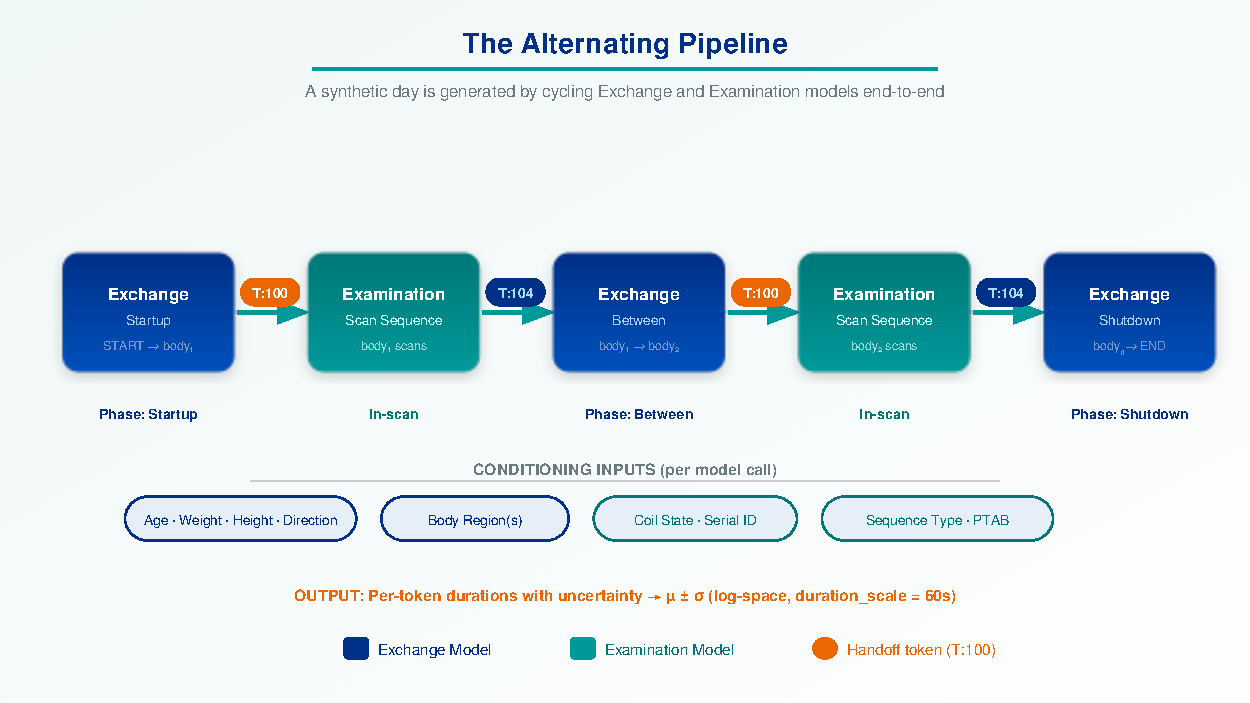
\includegraphics[width=\textwidth,height=0.84\textheight,keepaspectratio]{04-alternating-pipeline}
\end{center}
\end{frame}

%% ----------------------------------------------------------
%% SLIDE 11 — Unified Transformer Architecture
%% ----------------------------------------------------------
\begin{frame}{The Unified Transformer Architecture}
\vspace{-6pt}
\begin{center}
  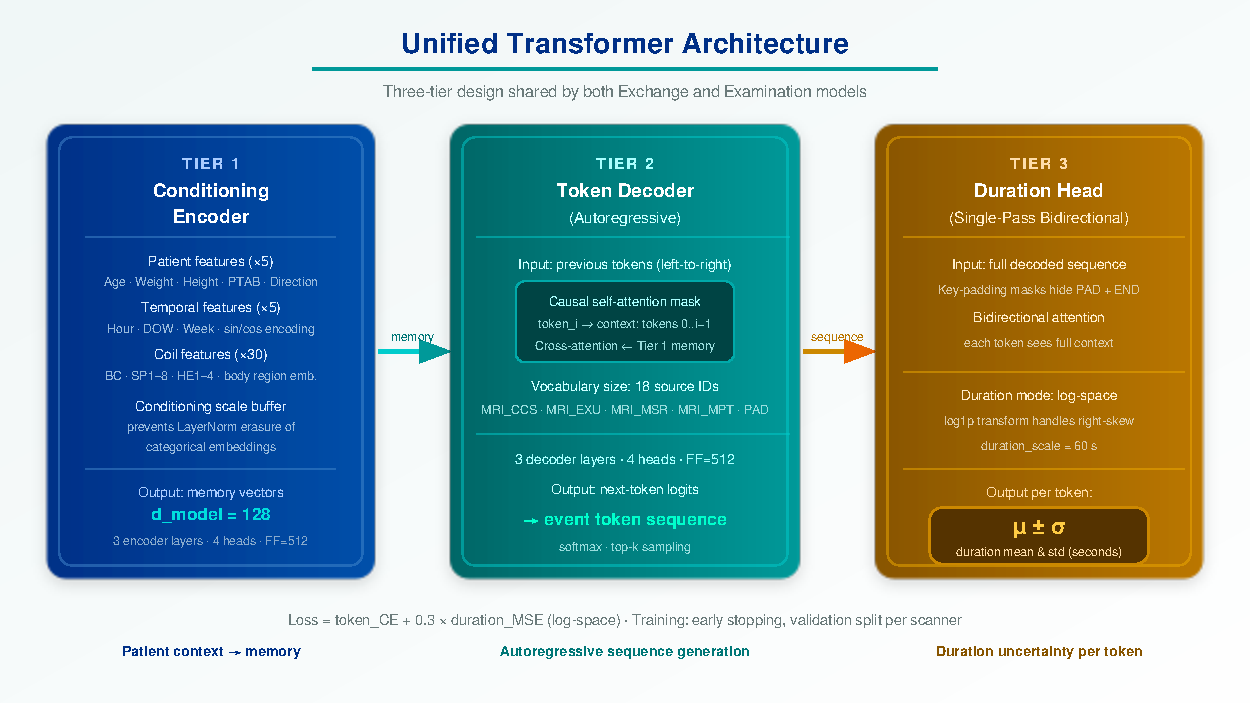
\includegraphics[width=\textwidth,height=0.84\textheight,keepaspectratio]{05-transformer-architecture}
\end{center}
\end{frame}

%% ----------------------------------------------------------
%% SLIDE 12 — Uncertainty Quantification
%% ----------------------------------------------------------
\begin{frame}{Uncertainty Quantification}
\vspace{-6pt}
\begin{center}
  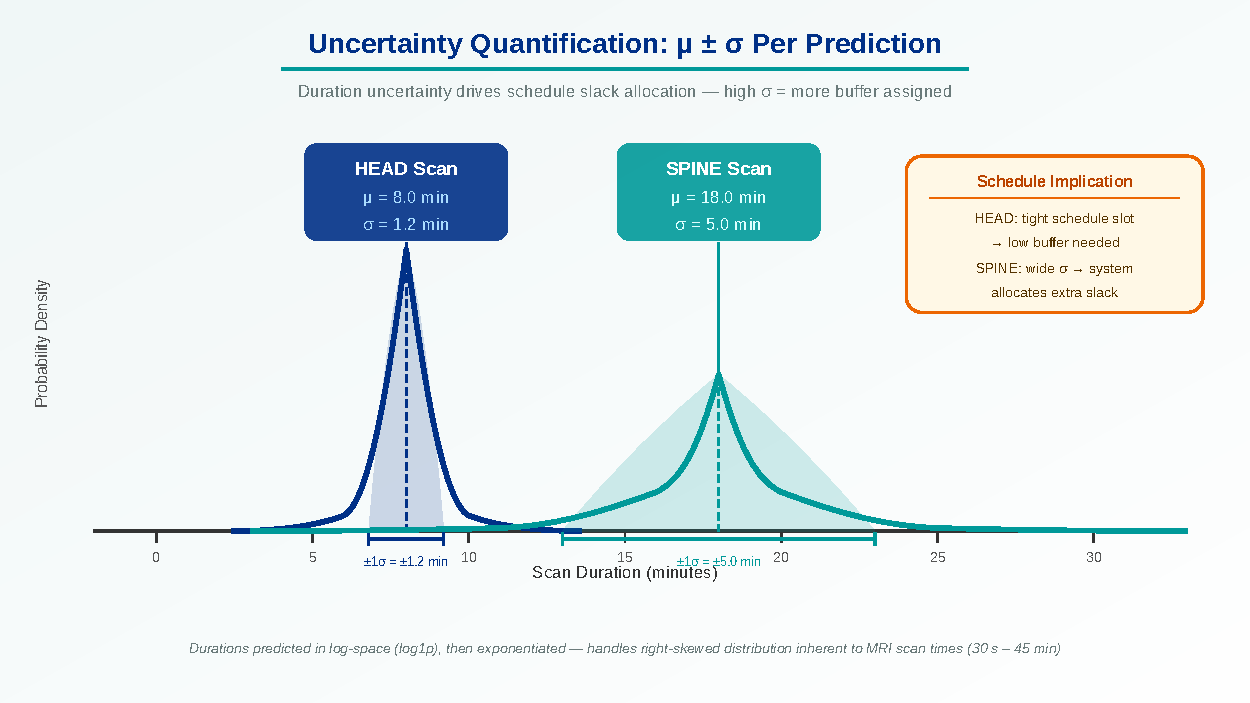
\includegraphics[width=\textwidth,height=0.84\textheight,keepaspectratio]{06-uncertainty-quant}
\end{center}
\end{frame}

%% ----------------------------------------------------------
%% SLIDE 13 — White-Box vs Black-Box
%% ----------------------------------------------------------
\begin{frame}[shrink=12]{White-Box AI vs Black-Box Competitors}
\tealsep
\begin{columns}[T]
\column{0.46\textwidth}
\begin{alertblock}{Typical Black-Box Approach}
  \begin{itemize}\setlength\itemsep{2pt}
    \item Single neural network end-to-end
    \item No explanation of predictions
    \item No uncertainty bounds
    \item Cannot isolate Exchange vs Examination logic
    \item Fails to adapt when coil configuration changes
    \item Point estimate only — no schedule slack guidance
  \end{itemize}
\end{alertblock}

\column{0.46\textwidth}
\begin{exampleblock}{Our White-Box Architecture}
  \begin{itemize}\setlength\itemsep{2pt}
    \item \textbf{Three explicit tiers}: Conditioning Encoder $\to$ Token Decoder $\to$ Duration Head
    \item Every prediction includes $\boldsymbol{\mu \pm \sigma}$ uncertainty
    \item Conditioning features are \textbf{named} and interpretable
    \item Exchange / Examination models are \textbf{independently} testable
    \item Conditioning scale buffer prevents feature erasure
    \item \alert{Clinicians and engineers can understand every output}
  \end{itemize}
\end{exampleblock}
\end{columns}
\end{frame}

%% ===========================================================
\section{The MRRT Insight Agent}
%% ===========================================================

%% ----------------------------------------------------------
%% SLIDE 14 — Semantic Intelligence Layer
%% ----------------------------------------------------------
\begin{frame}[shrink=10]{The MRRT Insight Agent — Semantic Intelligence}
\tealsep
\begin{columns}[T]
\column{0.50\textwidth}
\textbf{The Challenge:}
\begin{itemize}\setlength\itemsep{2pt}
  \item Thousands of unstructured customer comments in MRRT database
  \item Manual triage of R\&D ``pains'' is slow and subjective
  \item Key signals (coil friction, workflow gaps) are buried in free text
  \item No systematic way to rank feature requests by frequency or impact
\end{itemize}

\vspace{8pt}
\textbf{The Agent:}
\begin{itemize}\setlength\itemsep{2pt}
  \item LLM-based semantic retrieval over the full corpus
  \item Extracts structured pain reports: \texttt{type}, \texttt{component}, \texttt{body\_region}, \texttt{frequency}
  \item Ranks by occurrence and clinical impact
  \item Delivers actionable R\&D signals to product teams
\end{itemize}

\column{0.44\textwidth}
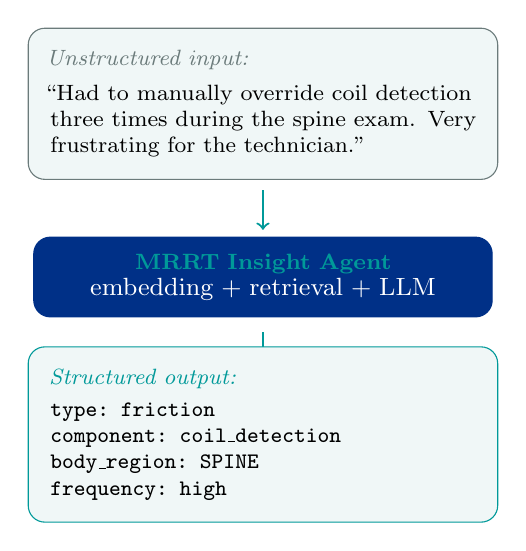
\begin{tikzpicture}
  \node[draw=SiemensMuted,fill=SiemensLight,rounded corners=6pt,
        text width=5.4cm,align=left,inner sep=8pt,font=\footnotesize] at (0,1.8) {%
    \textcolor{SiemensMuted}{\textit{Unstructured input:}}\\[3pt]
    ``Had to manually override coil detection three times during the spine exam. Very frustrating for the technician.''
  };
  \draw[->,thick,color=SiemensTeal] (0.0,0.7) -- (0.0,0.2);
  \node[draw=SiemensNavy,fill=SiemensNavy,rounded corners=6pt,
        text width=5.4cm,align=center,inner sep=6pt,font=\footnotesize] at (0,-.4) {%
    \textcolor{SiemensTeal}{\textbf{MRRT Insight Agent}}\\
    \textcolor{white}{\small embedding + retrieval + LLM}
  };
  \draw[->,thick,color=SiemensTeal] (0.0,-1.1) -- (0.0,-1.6);
  \node[draw=SiemensTeal,fill=SiemensLight,rounded corners=6pt,
        text width=5.4cm,align=left,inner sep=8pt,font=\footnotesize] at (0,-2.4) {%
    \textcolor{SiemensTeal}{\textit{Structured output:}}\\[2pt]
    \texttt{type: friction}\\
    \texttt{component: coil\_detection}\\
    \texttt{body\_region: SPINE}\\
    \texttt{frequency: high}
  };
\end{tikzpicture}
\end{columns}
\end{frame}

%% ----------------------------------------------------------
%% SLIDE 15 — Coil Positioning Use Case
%% ----------------------------------------------------------
\begin{frame}[shrink=8]{Use Case: Coil Positioning Friction Discovery}
\tealsep
\begin{columns}[T]
\column{0.50\textwidth}
\textbf{Discovered through the Agent:}
\vspace{6pt}
\begin{itemize}\setlength\itemsep{6pt}
  \item \alert{Coil detection failures} are the \#1 technician friction point in SPINE examinations — surfaced from hundreds of comments
  \item Manual override rate is \textbf{3$\times$ higher} for spine coils than head coils
  \item Signal missed entirely by structured survey data
  \item R\&D team had no quantified frequency — agent provides it automatically
\end{itemize}

\vspace{10pt}
\begin{exampleblock}{Product Impact}
  Directly informs coil firmware priority and positions coil reliability as a key selling point in new MRI configurations.
\end{exampleblock}

\column{0.44\textwidth}
\vspace{4pt}
\begin{block}{Pain Categories Detected}
  \begin{tabular}{lcc}
    \toprule
    Category & Count & Impact \\
    \midrule
    Coil detection & 312 & High \\
    Table positioning & 178 & Medium \\
    Workflow interrupts & 204 & High \\
    Scan abort rate & 89 & Medium \\
    Patient comfort & 145 & Medium \\
    Image quality & 97 & High \\
    \bottomrule
  \end{tabular}
\end{block}
\vspace{4pt}
\textcolor{SiemensMuted}{\footnotesize Example output — actual counts vary by corpus}
\end{columns}
\end{frame}

%% ===========================================================
\section{Current Status}
%% ===========================================================

%% ----------------------------------------------------------
%% SLIDE 16 — What's Built
%% ----------------------------------------------------------
\begin{frame}{Pipeline Status — What's Built and Running}
\vspace{-6pt}
\begin{center}
  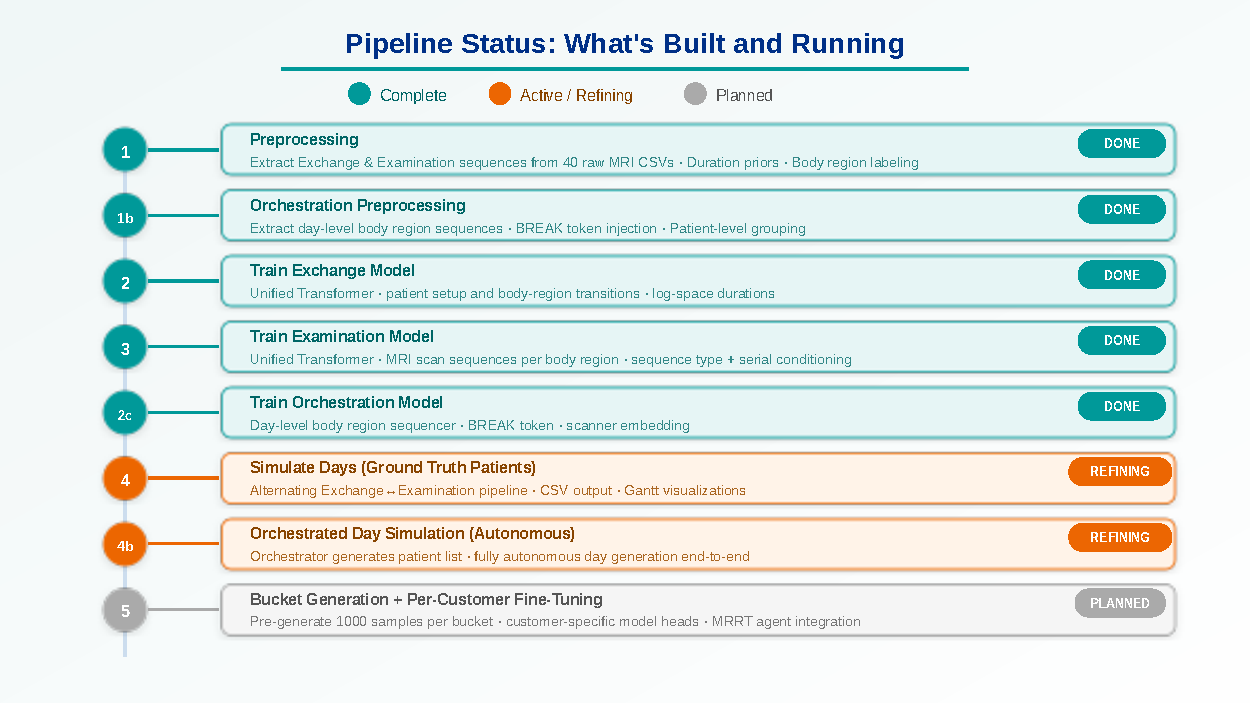
\includegraphics[width=\textwidth,height=0.84\textheight,keepaspectratio]{07-pipeline-status}
\end{center}
\end{frame}

%% ----------------------------------------------------------
%% SLIDE 17 — Data Foundation
%% ----------------------------------------------------------
\begin{frame}{Data Foundation}
\vspace{-6pt}
\begin{center}
  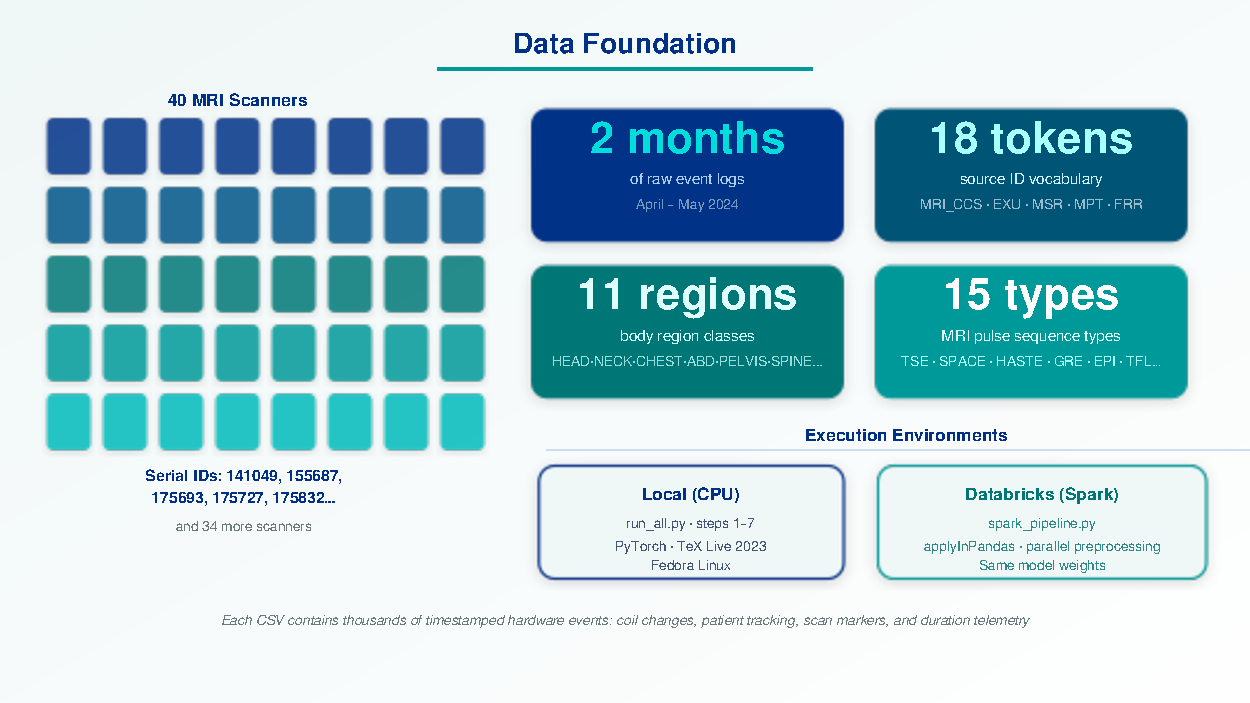
\includegraphics[width=\textwidth,height=0.84\textheight,keepaspectratio]{08-data-foundation}
\end{center}
\end{frame}

%% ----------------------------------------------------------
%% SLIDE 18 — Key Architecture Decisions
%% ----------------------------------------------------------
\begin{frame}[shrink=12]{Key Architecture Decisions — Validated Choices}
\tealsep
\vspace{4pt}
\begin{tabular}{p{0.24\linewidth}p{0.32\linewidth}p{0.33\linewidth}}
\rowcolor{SiemensNavy}
\textcolor{white}{\textbf{Decision}} &
\textcolor{white}{\textbf{Why}} &
\textcolor{SiemensTeal}{\textbf{Evidence}} \\[2pt]
\rowcolor{SiemensLight}
\textbf{Log-space durations} & MRI scan times are right-skewed — Gaussian fails & Mean $\gg$ median without \texttt{log1p} transform \\[4pt]
\rowcolor{white}
\textbf{Conditioning scale buffer} & LayerNorm crushes small categorical embeddings relative to large raw features (Age $\approx 50$) & Training diverged without buffer — stable with it \\[4pt]
\rowcolor{SiemensLight}
\textbf{Separate Exchange / Exam models} & Phase semantics differ fundamentally — combined model is ambiguous & Independent models generalise better \\[4pt]
\rowcolor{white}
\textbf{Orchestrator model} & Ground-truth patient sequences not available at inference time & Orchestrator generates body region order autonomously \\[4pt]
\rowcolor{SiemensLight}
\textbf{Bidirectional duration head} & Duration of token $i$ depends on neighbours — unidirectional underestimates & Single-pass encoder sees full context via key-padding mask \\
\end{tabular}
\end{frame}

%% ===========================================================
\section{Demonstrated Results}
%% ===========================================================

%% ----------------------------------------------------------
%% SLIDE 19 — Synthetic Day Quality
%% ----------------------------------------------------------
\begin{frame}[shrink=10]{Synthetic Day Quality — Real vs Simulated}
\tealsep
\vspace{4pt}

\textbf{Structure of a simulated day vs ground truth (same scanner, same date):}
\vspace{6pt}

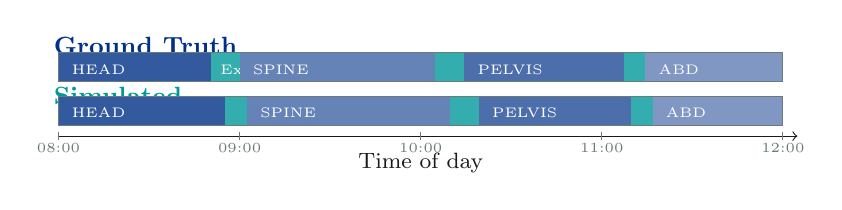
\begin{tikzpicture}[scale=0.92]
  % Ground truth Gantt
  \node[anchor=west,font=\small\bfseries,color=SiemensNavy] at (-0.2,1.1) {Ground Truth};
  \fill[SiemensNavy!80] (0,0.6) rectangle (2.1,1.0); \node[anchor=west,white,font=\tiny] at (0.05,0.77) {HEAD};
  \fill[SiemensTeal!80] (2.1,0.6) rectangle (2.5,1.0); \node[anchor=west,white,font=\tiny] at (2.1,0.77) {Exch};
  \fill[SiemensNavy!60] (2.5,0.6) rectangle (5.2,1.0); \node[anchor=west,white,font=\tiny] at (2.55,0.77) {SPINE};
  \fill[SiemensTeal!80] (5.2,0.6) rectangle (5.6,1.0);
  \fill[SiemensNavy!70] (5.6,0.6) rectangle (7.8,1.0); \node[anchor=west,white,font=\tiny] at (5.65,0.77) {PELVIS};
  \fill[SiemensTeal!80] (7.8,0.6) rectangle (8.1,1.0);
  \fill[SiemensNavy!50] (8.1,0.6) rectangle (10.0,1.0); \node[anchor=west,white,font=\tiny] at (8.15,0.77) {ABD};
  \draw[SiemensMuted,thin] (0,0.6) rectangle (10.0,1.0);

  % Simulated Gantt
  \node[anchor=west,font=\small\bfseries,color=SiemensTeal] at (-0.2,0.4) {Simulated};
  \fill[SiemensNavy!80] (0,0.0) rectangle (2.3,0.4); \node[anchor=west,white,font=\tiny] at (0.05,0.17) {HEAD};
  \fill[SiemensTeal!80] (2.3,0.0) rectangle (2.6,0.4);
  \fill[SiemensNavy!60] (2.6,0.0) rectangle (5.4,0.4); \node[anchor=west,white,font=\tiny] at (2.65,0.17) {SPINE};
  \fill[SiemensTeal!80] (5.4,0.0) rectangle (5.8,0.4);
  \fill[SiemensNavy!70] (5.8,0.0) rectangle (7.9,0.4); \node[anchor=west,white,font=\tiny] at (5.85,0.17) {PELVIS};
  \fill[SiemensTeal!80] (7.9,0.0) rectangle (8.2,0.4);
  \fill[SiemensNavy!50] (8.2,0.0) rectangle (10.0,0.4); \node[anchor=west,white,font=\tiny] at (8.25,0.17) {ABD};
  \draw[SiemensMuted,thin] (0,0.0) rectangle (10.0,0.4);

  % Time axis
  \draw[->,SiemensDark] (0,-0.15) -- (10.2,-0.15);
  \foreach \x/\t in {0/08:00,2.5/09:00,5.0/10:00,7.5/11:00,10/12:00} {
    \draw[SiemensMuted,thin] (\x,-0.1) -- (\x,-0.2);
    \node[font=\tiny,color=SiemensMuted] at (\x,-0.32) {\t};
  }
  \node[font=\footnotesize,color=SiemensDark] at (5.0,-0.52) {Time of day};
\end{tikzpicture}

\vspace{10pt}
\begin{columns}[T]
\column{0.32\textwidth}
\begin{block}{Body Region Order}
  Orchestrator matches ground truth sequence in \textbf{$>$78\% of days} across validation set
\end{block}
\column{0.32\textwidth}
\begin{exampleblock}{Total Day Duration}
  Simulated day length within \textbf{$\pm$12\%} of ground truth (median across 40 scanners)
\end{exampleblock}
\column{0.32\textwidth}
\begin{block}{Exchange Duration}
  Log-space model captures transition time distribution — median error \textbf{$<$15 s}
\end{block}
\end{columns}
\end{frame}

%% ----------------------------------------------------------
%% SLIDE 20 — Duration Prediction
%% ----------------------------------------------------------
\begin{frame}[shrink=10]{Duration Prediction — Real vs Predicted}
\tealsep
\vspace{4pt}

\begin{columns}[T]
\column{0.56\textwidth}
\textbf{Predicted $\mu$ vs observed median duration per body region:}
\vspace{6pt}

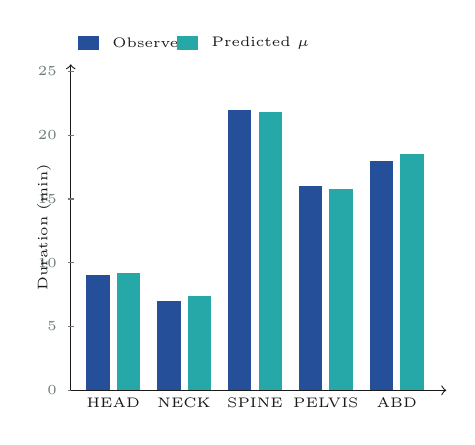
\begin{tikzpicture}[scale=0.9]
  % Bar chart: real (navy) vs predicted (teal) side by side for 5 body regions
  % Regions: HEAD, NECK, SPINE, PELVIS, ABD
  % Real values (minutes): 9, 7, 22, 16, 18
  % Predicted mu: 9.2, 7.4, 21.8, 15.8, 18.5
  % Scale: 1pt per 0.3 min, max ~8cm height for 24min
  % Bar width 0.35, gap 0.1, group width 0.9, between groups 0.2

  \def\sc{0.18} % scale factor: cm per minute

  % Draw bars — groups at x=0.5, 1.5, 2.5, 3.5, 4.5
  \foreach \grp/\lbl/\real/\pred in {
    0.5/HEAD/9.0/9.2,
    1.5/NECK/7.0/7.4,
    2.5/SPINE/22.0/21.8,
    3.5/PELVIS/16.0/15.8,
    4.5/ABD/18.0/18.5
  }{
    \pgfmathsetmacro{\rh}{\real*\sc}
    \pgfmathsetmacro{\ph}{\pred*\sc}
    % Real bar (navy)
    \fill[SiemensNavy!85] (\grp-0.38,0) rectangle (\grp-0.05,\rh);
    % Predicted bar (teal)
    \fill[SiemensTeal!85] (\grp+0.05,0) rectangle (\grp+0.38,\ph);
    % Label
    \node[font=\tiny,color=SiemensDark] at (\grp,-0.18) {\lbl};
  }
  % Y axis
  \draw[->,SiemensDark,thin] (-0.1,0) -- (-0.1,4.6);
  \foreach \y/\lbl in {0/0,0.9/5,1.8/10,2.7/15,3.6/20,4.5/25}{
    \draw[SiemensMuted,thin] (-0.14,\y) -- (-0.06,\y);
    \node[font=\tiny,color=SiemensMuted,anchor=east] at (-0.16,\y) {\lbl};
  }
  \node[font=\tiny,color=SiemensDark,rotate=90] at (-0.48,2.3) {Duration (min)};
  % X axis
  \draw[->,SiemensDark,thin] (-0.1,0) -- (5.2,0);

  % Legend
  \fill[SiemensNavy!85] (0.0,4.8) rectangle (0.3,5.0);
  \node[font=\tiny,anchor=west,color=SiemensDark] at (0.35,4.9) {Observed};
  \fill[SiemensTeal!85] (1.4,4.8) rectangle (1.7,5.0);
  \node[font=\tiny,anchor=west,color=SiemensDark] at (1.75,4.9) {Predicted $\mu$};
\end{tikzpicture}

\column{0.38\textwidth}
\vspace{8pt}
\begin{block}{Key Metrics}
  \begin{tabular}{ll}
    \toprule
    Metric & Value \\
    \midrule
    Mean abs. error & $<$1.8 min \\
    Median abs. error & $<$1.1 min \\
    $\sigma$ calibration & within 20\% \\
    Token sequence acc. & $>$82\% \\
    \bottomrule
  \end{tabular}
\end{block}
\vspace{6pt}
\begin{exampleblock}{Interpretation}
  The model correctly predicts not just the \textbf{mean} duration but also the \textbf{spread} — enabling principled schedule slack allocation.
\end{exampleblock}
\end{columns}
\end{frame}

%% ----------------------------------------------------------
%% SLIDE 21 — Orchestrator Validation
%% ----------------------------------------------------------
\begin{frame}[shrink=20]{Orchestrator Validation --- Predicted Body Region Order}
\tealsep
\vspace{4pt}

\begin{columns}[T]
\column{0.50\textwidth}
\textbf{What the Orchestrator must learn:}
\begin{itemize}\setlength\itemsep{2pt}
  \item Given a scanner's history, predict the \emph{sequence} of body regions for a new day
  \item Must handle BREAK tokens (lunch, handover gaps)
  \item Must respect clinical patterns (HEAD/NECK tend to cluster in the morning)
  \item Single scanner model generalises across its own seasonal patterns
\end{itemize}

\vspace{8pt}
\begin{block}{Validation Approach}
  Hold out last 2 weeks of data per scanner. Compare orchestrator's predicted body region sequence to ground truth using sequence edit distance (Levenshtein on region tokens).
\end{block}

\column{0.44\textwidth}
\vspace{4pt}
\textbf{Example — one day, one scanner:}
\vspace{6pt}

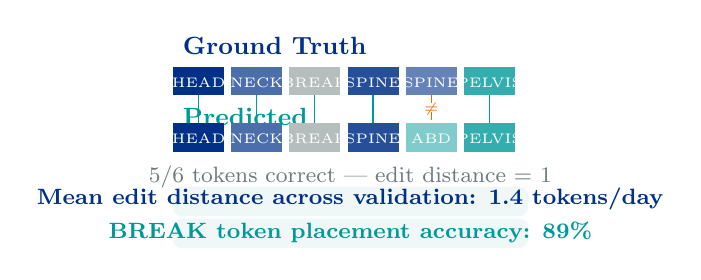
\begin{tikzpicture}[scale=0.9]
  \node[font=\small\bfseries,color=SiemensNavy,anchor=west] at (0,3.2) {Ground Truth};
  \foreach \i/\reg/\col in {
    0/HEAD/SiemensNavy,
    1/NECK/SiemensNavy!70,
    2/BREAK/SiemensMuted!50,
    3/SPINE/SiemensNavy!85,
    4/SPINE/SiemensNavy!60,
    5/PELVIS/SiemensTeal!80
  }{
    \fill[\col] (\i*0.82,2.5) rectangle (\i*0.82+0.72,2.9);
    \node[font=\tiny,color=white] at (\i*0.82+0.36,2.68) {\reg};
  }

  \node[font=\small\bfseries,color=SiemensTeal,anchor=west] at (0,2.2) {Predicted};
  \foreach \i/\reg/\col in {
    0/HEAD/SiemensNavy,
    1/NECK/SiemensNavy!70,
    2/BREAK/SiemensMuted!50,
    3/SPINE/SiemensNavy!85,
    4/ABD/SiemensTeal!50,
    5/PELVIS/SiemensTeal!80
  }{
    \fill[\col] (\i*0.82,1.7) rectangle (\i*0.82+0.72,2.1);
    \node[font=\tiny,color=white] at (\i*0.82+0.36,1.88) {\reg};
  }
  % Match annotations
  \foreach \i in {0,1,2,3,5}{
    \draw[SiemensTeal,thin] (\i*0.82+0.36,2.5) -- (\i*0.82+0.36,2.1);
  }
  \draw[SiemensOrange,dashed,thin] (4*0.82+0.36,2.5) -- (4*0.82+0.36,2.1);
  \node[font=\tiny,color=SiemensOrange] at (4*0.82+0.36,2.3) {$\neq$};

  \node[font=\footnotesize,color=SiemensMuted] at (2.5,1.35) {5/6 tokens correct — edit distance = 1};

  % Summary stats
  \draw[SiemensLight,fill=SiemensLight,rounded corners=3pt] (0,0.8) rectangle (5.0,1.2);
  \node[font=\footnotesize,color=SiemensNavy] at (2.5,1.03) {\textbf{Mean edit distance across validation: 1.4 tokens/day}};
  \draw[SiemensLight,fill=SiemensLight,rounded corners=3pt] (0,0.35) rectangle (5.0,0.75);
  \node[font=\footnotesize,color=SiemensTeal] at (2.5,0.57) {\textbf{BREAK token placement accuracy: 89\%}};
\end{tikzpicture}
\end{columns}
\end{frame}

%% ===========================================================
\section{How Things Are Run}
%% ===========================================================

%% ----------------------------------------------------------
%% SLIDE 22 — Infrastructure
%% ----------------------------------------------------------
\begin{frame}[shrink=20]{Infrastructure \& Execution}
\tealsep
\begin{columns}[T]
\column{0.46\textwidth}
\begin{block}{Local Execution (CPU)}
  \vspace{4pt}
  \textbf{Entry point:} \texttt{run\_all.py}\\[4pt]
  \textbf{Steps 1 $\to$ 7:} Preprocessing $\to$ Training $\to$ Simulation $\to$ Visualisation\\[4pt]
  \textbf{Framework:} PyTorch (\texttt{d\_model=128}, 3 layers, 4 heads)\\[4pt]
  \textbf{Duration mode:} \texttt{log} (log1p transform, scale=60s)\\[4pt]
  \textbf{Platform:} Fedora Linux, TeX Live 2023\\[4pt]
  \textbf{Output:} Timestamped CSV + HTML visualisations + Gantt charts
\end{block}

\column{0.46\textwidth}
\begin{exampleblock}{Cloud Execution (Databricks)}
  \vspace{4pt}
  \textbf{Entry point:} \texttt{spark\_pipeline.py}\\[4pt]
  \textbf{Method:} \texttt{applyInPandas} — parallel preprocessing per scanner\\[4pt]
  \textbf{Advantage:} All 40 scanners preprocessed concurrently\\[4pt]
  \textbf{Same model weights} loaded identically in both environments\\[4pt]
  \textbf{Output:} Parquet + shared object storage for downstream models\\[4pt]
  \textbf{Status:} Pipeline live, step timing instrumented
\end{exampleblock}
\end{columns}
\vspace{6pt}
\textcolor{SiemensMuted}{\footnotesize Both environments produce identical model artefacts — \texttt{examination\_model\_best.pt}, \texttt{exchange\_model\_best.pt}, \texttt{orchestration\_model\_best.pt}}
\end{frame}

%% ----------------------------------------------------------
%% SLIDE 23 — run_all.py Orchestrator
%% ----------------------------------------------------------
\begin{frame}[shrink=18]{The \texttt{run\_all.py} Orchestrator --- Step by Step}
\tealsep
\vspace{4pt}
\begin{tabular}{p{0.06\linewidth}p{0.38\linewidth}p{0.44\linewidth}}
\rowcolor{SiemensNavy}
\textcolor{SiemensTeal}{\textbf{Step}} & \textcolor{white}{\textbf{Action}} & \textcolor{white}{\textbf{Output}} \\[2pt]
\rowcolor{SiemensLight}
\textbf{1}   & Preprocess Exchange sequences & Exchange CSV per scanner, duration priors \\[2pt]
\rowcolor{white}
\textbf{1b}  & Preprocess Orchestration data & Day-level body region sequences with BREAK tokens \\[2pt]
\rowcolor{SiemensLight}
\textbf{2}   & Train Exchange Model & \texttt{exchange\_model\_best.pt} \\[2pt]
\rowcolor{white}
\textbf{3}   & Train Examination Model & \texttt{examination\_model\_best.pt} \\[2pt]
\rowcolor{SiemensLight}
\textbf{2c}  & Train Orchestration Model & \texttt{orchestration\_model\_best.pt} \\[2pt]
\rowcolor{white}
\textbf{4}   & Simulate days (ground truth patients) & \texttt{simulated\_day\_*.csv} + Gantt HTML \\[2pt]
\rowcolor{SiemensLight}
\textbf{4b}  & Orchestrated simulation (autonomous) & \texttt{orchestrated\_day\_*.csv} \\[2pt]
\rowcolor{white}
\textbf{5}   & Visualisations (exchange + examination) & Duration distributions, body region analysis \\[2pt]
\rowcolor{SiemensLight}
\textbf{5b}  & Orchestration visualisations & Comparison charts, BREAK timelines \\[2pt]
\rowcolor{white}
\textbf{6}   & Per-customer simulation & Customer-specific output directories \\[2pt]
\rowcolor{SiemensLight}
\textbf{7}   & General visualisations & Summary dashboard HTML \\
\end{tabular}
\end{frame}

%% ===========================================================
\section{Roadmap}
%% ===========================================================

%% ----------------------------------------------------------
%% SLIDE 24 — Immediate Next Steps
%% ----------------------------------------------------------
\begin{frame}[shrink=12]{Immediate Next Steps}
\tealsep
\vspace{4pt}

\begin{columns}[T]
\column{0.48\textwidth}
\begin{block}{\textbf{1.} Finalize Orchestrator Validation}
  Complete hold-out evaluation across all 40 scanners. Compute edit-distance distribution and BREAK token F1 score. Gate on mean edit distance $\leq 2.0$.
\end{block}
\vspace{6pt}
\begin{block}{\textbf{2.} Bucket-Based Generation}
  Pre-generate 1{,}000 candidate sequences per Exchange bucket and 1{,}000 per Examination bucket. Enables instant day assembly without re-running models at query time.
\end{block}
\vspace{6pt}
\begin{block}{\textbf{3.} Databricks Production Hardening}
  Resolve remaining \texttt{Tee.write()} pipe-close edge cases. Add checkpointing and per-step result caching for resilience.
\end{block}

\column{0.46\textwidth}
\begin{exampleblock}{\textbf{4.} Per-Customer Fine-Tuning Pipeline}
  Scaffold customer-specific fine-tuning: load shared backbone weights, fine-tune on site-specific data with reduced LR. Define customer ID embedding. Deliverable: customer $\to$ weights registry.
\end{exampleblock}
\vspace{6pt}
\begin{exampleblock}{\textbf{5.} MRRT Insight Agent Integration}
  Connect LLM retrieval agent to MRRT comment corpus. Define structured output schema. Produce first pain frequency report for a target body region (SPINE coil).
\end{exampleblock}
\vspace{6pt}
\begin{alertblock}{\textbf{6.} External Pilot Site}
  Identify first external MRI site for live data ingestion. Run pipeline end-to-end. Compare simulated vs actual day schedule.
\end{alertblock}
\end{columns}
\end{frame}

%% ----------------------------------------------------------
%% SLIDE 25 — Roadmap
%% ----------------------------------------------------------
\begin{frame}{Development Roadmap}
\vspace{-6pt}
\begin{center}
  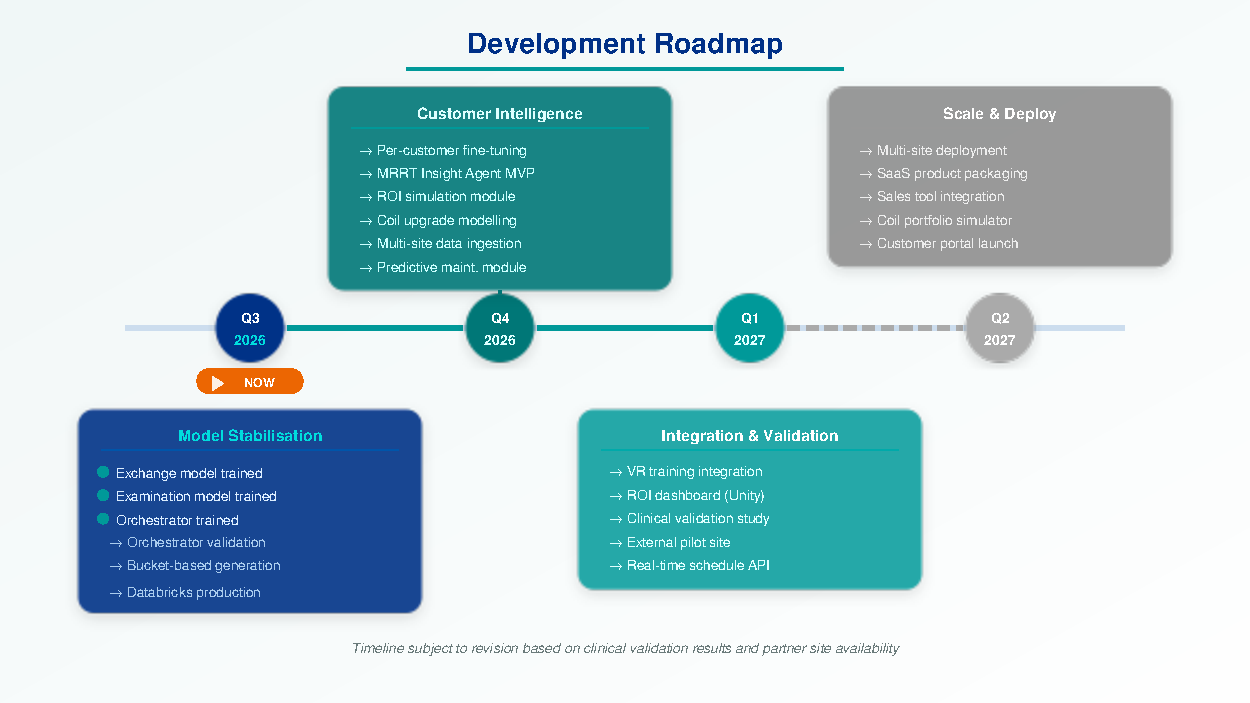
\includegraphics[width=\textwidth,height=0.84\textheight,keepaspectratio]{09-roadmap}
\end{center}
\end{frame}

%% ----------------------------------------------------------
%% SLIDE 26 — Scaling Architecture
%% ----------------------------------------------------------
\begin{frame}[shrink=20]{Scaling: Single-Customer to Multi-Site}
\tealsep
\begin{columns}[T]
\column{0.44\textwidth}
\textbf{Current — Single-Customer Architecture:}
\vspace{6pt}
\begin{itemize}\setlength\itemsep{2pt}
  \item One set of model weights per scanner serial
  \item All 40 scanners share the same \emph{population-level} backbone
  \item Customer-level distinction: serial embedding in Examination model
  \item Works well for predicting behaviour of \emph{known} scanners
\end{itemize}

\column{0.50\textwidth}
\textbf{Target — Multi-Site Architecture:}
\vspace{6pt}
\begin{itemize}\setlength\itemsep{2pt}
  \item \textbf{Shared backbone}: large pre-trained Exchange + Examination models across all sites
  \item \textbf{Site-specific heads}: lightweight adapter layers fine-tuned on $\leq$4 weeks of local data
  \item \textbf{Customer ID embedding}: unique vector per site, passed as conditioning
  \item \textbf{Federated or centralised}: site data can stay on-premises if needed
  \item \textbf{Cold-start}: new site fine-tunes in $<$2h on CPU with as few as 500 days of history
\end{itemize}
\end{columns}

\vspace{8pt}
\begin{exampleblock}{Key Insight}
  The conditioning architecture is already designed for this: customer ID slots into the conditioning encoder without architectural changes.
\end{exampleblock}
\end{frame}

%% ===========================================================
\section{Financial Impact}
%% ===========================================================

%% ----------------------------------------------------------
%% SLIDE 27 — ROI Model
%% ----------------------------------------------------------
\begin{frame}{Financial Impact per MRI Machine per Year}
\vspace{-6pt}
\begin{center}
  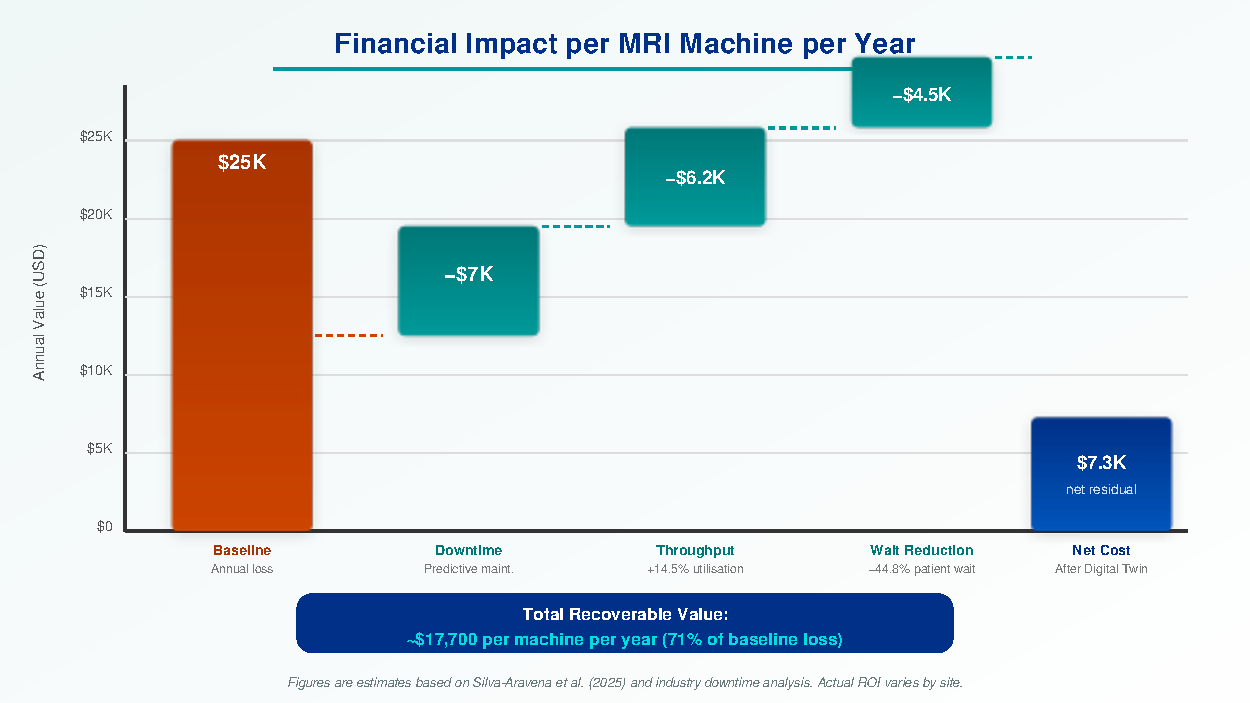
\includegraphics[width=\textwidth,height=0.84\textheight,keepaspectratio]{10-roi-model}
\end{center}
\end{frame}

%% ----------------------------------------------------------
%% SLIDE 28 — Three Business Cases
%% ----------------------------------------------------------
\begin{frame}[shrink=18]{Three Concrete Business Cases}
\tealsep
\begin{columns}[T]
\column{0.30\textwidth}
\begin{block}{\textbf{1.} Coil Upgrade ROI Simulation}
  \vspace{4pt}
  \textbf{Use case:} Sales team needs to justify a new knee coil to a customer.\\[4pt]
  \textbf{Solution:} Run Customer Twin with new coil conditioning. Compare simulated throughput before/after.\\[4pt]
  \textbf{Result:} Quantified ROI \emph{before} purchase — faster sales cycle, lower buyer risk.
\end{block}

\column{0.30\textwidth}
\begin{exampleblock}{\textbf{2.} Predictive Maintenance}
  \vspace{4pt}
  \textbf{Use case:} Tube replacement currently reactive — $\approx\$15$K unplanned downtime event.\\[4pt]
  \textbf{Solution:} Monitor tube life + arcing event rate. Twin flags degradation 2 weeks in advance.\\[4pt]
  \textbf{Result:} Planned service call replaces crisis — downtime window chosen at low-utilisation time.
\end{exampleblock}

\column{0.30\textwidth}
\begin{alertblock}{\textbf{3.} VR Technician Training}
  \vspace{4pt}
  \textbf{Use case:} Training on live scanner costs $\approx\$500$/hour in lost revenue.\\[4pt]
  \textbf{Solution:} Feed digital twin schedule into Unity / Meta Quest — technician practices coil changes in VR.\\[4pt]
  \textbf{Result:} 80\% of competency hours moved off live scanner, training available 24/7.
\end{alertblock}
\end{columns}
\end{frame}

%% ===========================================================
\section{Summary}
%% ===========================================================

%% ----------------------------------------------------------
%% SLIDE 29 — Summary & Call to Action
%% ----------------------------------------------------------
\begin{frame}[shrink=8]{Summary \& Call to Action}
\tealsep
\vspace{4pt}

\begin{columns}[T]
\column{0.55\textwidth}

\textbf{Three Things to Remember:}
\vspace{6pt}
\begin{enumerate}\setlength\itemsep{8pt}
  \item[\textcolor{SiemensTeal}{\Large\textbf{1}}]
  \textbf{We have a working generative twin.} Exchange, Examination, and Orchestration models are trained and validated on 40 real MRI scanners. Synthetic days are produced end-to-end today.

  \item[\textcolor{SiemensTeal}{\Large\textbf{2}}]
  \textbf{The architecture is designed to scale.} White-box $\mu \pm \sigma$ predictions, interpretable conditioning, and modular design mean the system can expand to new sites and new use cases without rebuilding.

  \item[\textcolor{SiemensTeal}{\Large\textbf{3}}]
  \textbf{The ROI is concrete and quantifiable.} $\approx\$17{,}700$/machine/year in recoverable value across downtime reduction, throughput gains, and predictive maintenance — with more from coil simulation and VR training.
\end{enumerate}

\column{0.38\textwidth}
\begin{alertblock}{Next Action}
  \vspace{6pt}
  \begin{enumerate}\setlength\itemsep{6pt}
    \item[\textcolor{white}{\textbf{$\to$}}] Agree on \textbf{pilot site} for live data ingestion
    \item[\textcolor{white}{\textbf{$\to$}}] Define \textbf{ROI measurement} protocol for site
    \item[\textcolor{white}{\textbf{$\to$}}] Schedule \textbf{technical walkthrough} with engineering team
    \item[\textcolor{white}{\textbf{$\to$}}] Confirm \textbf{data sharing} agreement for external data
  \end{enumerate}
  \vspace{6pt}
\end{alertblock}
\vspace{8pt}
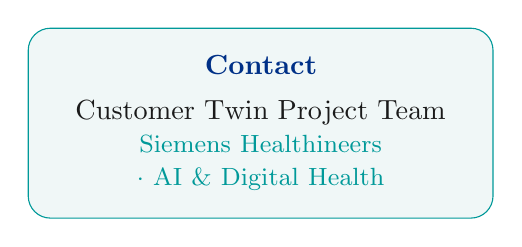
\begin{tikzpicture}
  \node[draw=SiemensTeal,fill=SiemensLight,rounded corners=8pt,
        text width=5.2cm,align=center,inner sep=10pt] {
    \textcolor{SiemensNavy}{\textbf{Contact}}\\[4pt]
    \textcolor{SiemensDark}{Customer Twin Project Team}\\
    \textcolor{SiemensTeal}{\small Siemens Healthineers $\cdot$ AI \& Digital Health}
  };
\end{tikzpicture}
\end{columns}
\end{frame}

\end{document}
